%
\chapter[Procesos Quimicos en la Atmosfera]{Procesos qu\'{\i}micos en la atm\'osfera}

Los procesos químicos en la atmósfera son el motor de transformación de los compuestos emitidos por fuentes naturales y actividad \gloss[word]{antropica}, determinando su impacto ambiental y ciclo de vida. Este capítulo explora las reacciones clave que gobiernan la dinámica de contaminantes en diferentes capas atmosféricas, con énfasis en mecanismos de oxidación, interacciones fotoquímicas y transformación de especies críticas.

En la Sección~\ref{7quim}, se analiza la \textbf{oxidación atmosférica}, proceso fundamental que regula la degradación de contaminantes. Se describe la cadena de oxidación (\ref{71cox}), donde radicales libres como \ce{OH^.} actúan como ``detergentes atmosféricos'', y la vida química de los compuestos orgánicos volátiles (COVs) (\ref{72cov}), clave para entender su persistencia y formación de ozono troposférico.

Las \textbf{Secciones \ref{qs02} y \ref{qno2}} profundizan en la química de dos contaminantes críticos:
\begin{itemize}
    \item \textbf{Dióxido de azufre (\ce{SO2})}: Su conversión a ácido sulfúrico (\ce{H2SO4}) mediante reacciones heterogéneas (\ref{qs02} ) y el papel de los compuestos reducidos de azufre (\ref{crso2}) en la nucleación de aerosoles.
    \item \textbf{Dióxido de nitrógeno (\ce{NO2})}: Su rol en el ciclo del ozono (\ref{cozono}), actuando como precursor tanto en la formación de smog como en la destrucción estratosférica de ozono (\ce{O3}).
\end{itemize}

Las Secciones~\ref{raminas} a  \ref{rchal} abordan la reactividad de grupos funcionales específicos:
\begin{itemize}
    \item \textbf{Aminas} (\ref{raminas}): Neutralización de ácidos en nubes y formación de nanopartículas
    \item \textbf{Compuestos de carbono} (\ref{recc}): Oxidación de metano (\ce{CH4}) y hidrocarburos aromáticos
    \item \textbf{Halógenos} (\ref{rchal}): Destrucción catalítica de ozono estratosférico (Ej.: \ce{Cl^.} de CFCs)
\end{itemize}

Estos procesos explican fenómenos globales como la lluvia ácida, el agotamiento de la capa de ozono y el cambio climático, demostrando cómo interacciones moleculares escalan a impactos planetarios. El estudio integrado de estas reacciones provee herramientas para modelar escenarios de contaminación y diseñar estrategias de mitigación.

\section{Oxidación en la atmósfera}
\index{atmosfera@atmósfera!oxidacion@oxidación}\label{7quim}

La atmósfera es un ambiente oxidante: un hidrocarburo emitido puede oxidarse varias veces para formar los productos finales \ce{CO2} y \ce{H2O}. Los tres oxidantes principales son el radical hidroxilo\index{hidroxilo} (\ce{OH}), el ozono\index{ozono} (\ce{O3 }) y el nitrato\index{nitrato} (\ce{NO3}) (clasificados según su fuerza de oxidación decreciente).  Las reacciones de oxidación desempeñan un papel clave en la limpieza de la atmósfera (de lo contrario, las concentraciones de hidrocarburos serían demasiado altas ).

En primera aproximación, la capacidad oxidante de la atmósfera viene dada por la concentración de OH (unas $10^6$ moléculas cm${^{-3}}$ en la troposfera).

El radical hidroxilo OH a veces se denomina ``depurador químico', de la atmósfera. La mayor parte de los procesos de oxidación tienen lugar en las regiones tropicales.

El ozono (\ce{O3})  juega un papel decisivo para la producción de OH a través de su fotólisis,

\reaction{ O3 + h\nu (\lambda \leqslant 310 nm) ->[L_1] O2 + O(^1D) \label{RA}}

El estado excitado de los átomos de oxígeno, \ce{O(^1D)}, puede estabilizarse en la forma \ce{O(^3P)}, con la reacción

\reaction{ O(^1D) + M ->[k_2] O2 +   O(^3P) + M \label{RB}}

o producir OH con la reacción

\reaction{ O(^1D) + H2O  ->[k_3] O2 +  2OH \label{RC}}
El punto clave es que sólo el estado fundamental excitado \ce{O(^1D)} reacciona con el vapor de agua (un compuesto estable). Como resultado, la producción de OH está directamente relacionada con la fotólisis del ozono.

La reacción global resultante de estas tres reacciones es

\reaction{ O3 ->[h\nu, \ce{H2O}] 2OH \label{RD}}

Reglas que pueden ayudar y simplificar la forma de calcular los estados de oxidación\footnote{\textbf{Nota sobre oxidación}: Si un elemento pierde electrones, hay más protones que electrones en el átomo, por lo que tendrá una carga positiva; por lo tanto, presentará un estado de oxidación positivo. Si gana electrones, hay más electrones que protones en el átomo, por lo que su carga y estado de oxidación serán negativos.}:
\begin{enumerate}
\item El estado de oxidación de todos los elementos en su estado libre es 0. Esto se debe a que el elemento no ha perdido ni ganado electrones y, por tanto, es neutro. Este es el caso de los metales puros o las moléculas biatómicas.

Por ejemplo: Zn, H y Cl.
\item La suma de los estados de oxidación de todos los átomos o iones de un compuesto neutro es igual a 0.

Por ejemplo: en el NaCl, el estado de oxidación del Na es +1 y el del Cl es -1. La suma de estos números da como resultado 0.
\item La suma de los estados de oxidación de un ion es igual a su carga. Esto se aplica tanto a los iones monoméricos como a los complejos.

Por ejemplo: el estado de oxidación del ion monoatómico de Flúor (\ce{F-}) es -1.

Por ejemplo: en el ion \ce{CO3^{-2}}, el C tiene un estado de oxidación de +4 y los tres O tienen un estado de oxidación de -2. Entonces, 4 + 3 (-2) = -2, que es la carga del ion.
\item En un ion o en un compuesto, el elemento más electronegativo suele tener el estado de oxidación más negativo. Tener presente que en la tabla periódica la electronegatividad\index{electronegatividad} aumenta de izquierda a derecha en un período y disminuye de arriba hacia abajo en un grupo.

Por ejemplo: en el \ce{F2O}, el F es más electronegativo que el oxígeno, por lo que tiene el estado de oxidación más negativo. Aquí, el F tiene un estado de oxidación de -1 y el O tiene un estado de oxidación de +2.
\end{enumerate}

\subsection{La cadena de oxidación}\index{oxidacion@oxidación!cadena de}\label{71cox}
Las reacciones más frecuentes implican radicales con electrones libres en la capa de valencia externa (lo que implica que son altamente reactivos), como OH o \ce{HO2}.

Una cadena de oxidación se puede dividir en la siguiente secuencia de pasos sucesivos:

\begin{description}
\item[Iniciación ] Una especie estable (no es un radical; escrito como \ce{X_{norad}}) se disocia mediante una reacción fotolítica, que conduce a la producción de al menos un radical (\ce{X_{rad}}):
\reaction{X_{norad} +  h$\nu$  ->  X_{rad} \label{R1} }
La fotólisis del ozono (\ref{RA}) es un ejemplo de esta etapa.
\item[Propagación ] Los radicales resultantes reaccionan con especies estables (se mantiene la notación \ce{X_{norad}}, aunque no necesariamente sean las mismas especies que antes). Los nuevos radicales (también escritos como \ce{X_{rad}}) se producen mediante reacciones de oxidación:
\reaction{X_{norad}  +  X_{rad}  -> X_{norad}  +  X_{rad}  \label{R2}}
\item[Reacción de ramificación]  Las especies estables pueden disociarse durante una reacción fotolítica y pueden generar otros radicales con reacciones similares a (\ref{R1}).
\item[Terminación ] Los radicales pueden reaccionar entre ellos para producir una especie estable, lo que finaliza la cadena de oxidación:

\reaction{X_{rad}  +  X_{rad}  -> X_{norad}    }
\end{description}

Las especies estables que se oxidan durante la etapa de propagación (\ref{R2}) deben considerarse como un ``combustible''  para la oxidación, ya que participan en la producción de radicales. Normalmente es el caso de los COV, CO y \ce{CH4}.

\subsection{La vida química de compuestos orgánicos volátiles}\label{72cov}

La vida química de algunos compuestos orgánicos volátiles (COV)\index{COV} se muestra en el \textbf{Cuadro~\ref{tvcov}}. Se calculan con respecto a las especies oxidantes OH, \ce{O3} y \ce{NO3}, usando una ecuación similar a 
\begin{equation*}
\tau=\frac{1}{k_{\ce{OH}],i}[\ce{OH}]}
\end{equation*}
(Como era de esperar, la vida química aumenta cuando la concentración de OH disminuye y cuando $k_{\ce{OH}],i}$ disminuye, es decir, cuando la especie es menos reactiva.)
\begin{table}[htp]
\caption[Vida Química para algunos COV]{Vida Química para algunos compuestos orgánicos volátiles  a 298\kelvin \footnotesize{(d para día, h para hora y min para minuto)}}
\begin{center}
\begin{tabular}{|l|c|c|c|}\hline
Especie & Oxidación  &  Oxidación  &  Oxidación  \\
              &  con OH    & con \ce{O3} & con \ce{NO3} \\\hline
metano & 1837 d &  -- & -- \\
etano   & 48 d &  -- & 2960 d \\
butano & 4.8 d &  -- & 391 d \\
eteno & 1.4 d &  6.7 d & 107 d \\
propeno & 10.6 h & 1.1 d & 2.3 d\\
isopreno & 2.8 h & 20.2 h & 45 min \\
$\beta-$pineno & 3.5 h & 17.2 h & 12 min \\\hline
\end{tabular}
\end{center}
\label{tvcov}
\end{table}%
Las reacciones con OH suelen ser las más rápidas y, como consecuencia, controlan la vida química. Es fácil comprobar que el aumento de la ``complejidad química'' da como resultado un aumento de la reactividad y, por tanto, una disminución de la vida útil.

\section{Química del dióxido de azufre}\label{qs02}
\index{SO2@\ce{SO2}!quimica@química}
Desde le punto termodinámico, el dióxido de azufre (\ce{SO2}) posee una fuerte tendencia a reaccionar con el oxígeno del aire.
\reaction{2SO2 +O2 -> 2SO3 \label{RS1}}

La proporción de concentraciones en equilibrio de [\ce{SO3}]/[\ce{SO2}] \index{SO2@\ce{SO2}} \index{azufre!oxidos@\'oxidos} es cerca de $8\times10^{11}$ en aire a 1 atmósfera y 25\celsius. Sin embargo la rapidez de reacción de la reacción~\ref{RS1}  es muy baja en fase gas en una atmósfera libre de catalizadores por lo que se puede descartar como fuente de \ce{SO3}. Una vez formado el \ce{SO3}  reacciona muy rápidamente con el vapor de agua par formar el ácido sulfúrico 

\reaction{ SO3  + H2O -> H2SO4(ac) \label{RS2}}
cualquier proceso en el que el \ce{SO3} se forme en una atmósfera húmeda pude considerarse equivalente a la formación del \ce{H2SO4}.

Para explica la oxidación del \ce{SO2}, uno debe ver las reacciones diferentes a la directa. El dióxido de azufre absorbe la luz en la región ultravioleta de  la luz solar incidente en la troposfera, llevan a un estado exitado a la molécula de \ce{SO2}.
\reaction{ SO2  + h$\nu$ -> SO2^* }
El estado exitado del \ce{SO2^*}, está no disociado. S\'olo longitudes de onda debajo de los 218 nm, los cuales no penetran a la troposfera, proveen la energía suficiente para permitir la fotodisociación de \ce{SO2}. Si cada molécula que \ce{SO2} que queda fotoexitada se oxidase mediante la reacción con el \ce{O2} u otra especie, se tendría que la vida del \ce{SO2} es tan baja como de 52 min. Sin embargo, conocemos que el tiempo de vida del \ce{SO2} es mucho mayor que eso.

El  \ce{SO2} reacciona en condiciones de la troposfera via procesos fase gas y acuosa y se remueve fisicamente via deposito seco y húmedo. Con respecto a la reacción fase gas, la reacción con el OH es la dominante:
\reaction{ SO2  + OH^. +  M ->  HOSO2^. + M }
seguido de la regeneración del radical \ce{HO2}\index{radical!HO2@\ce{HO2}}
\reaction{  HOSO2^. + O2 -> HO2^.  + SO3 }
\reaction{  HO2^. + NO -> NO2  + OH^. }
y el trióxido se convierte a ácido sulfúrico via la reacción \ref{RS2}:
\reaction*{ SO3  + H2O -> H2SO4} 
El tiempo de vida del \ce{SO2} basado en la reacción con el radical OH, a concentraciones típicas atmosférIcas, es de cerca a una semana. El \ce{SO2} es uno de los gases que se remueve de forma razonablemente eficiente de la atmósfera por depósito seco.

\subsection{Compuestos reducidos de azufre}\index{azufre!compuestos reducidos}\label{crso2}
Las especies reducidas de azufre  RSR' reacciona con los radicales OH y \ce{NO3}. Éstas son emitidas por procesos biogénicos liberando especies como monosulfuro de carbono (CS), ácido sulfhídrico (\ce{H2S}), sulfuro de carbonilo (COS), dimetil sulfuro (\ce{CH3SCH3} o DMS) y disulfuro de metilo (\ce{CH3SSCH3}). Para el \ce{H2S}, el proceso troposférico dominante de remoción involucra a la reacción del radical OH,

\reaction{ H2S  + OH^.  ->  SH^. + H2O }

El tiempo de vida del \ce{H2S} por esta reacción es cerca de 70 horas. Parece que el radical \ce{SH^.} sigue una serie de reacciones resultado en la formación de  \ce{SO2}. Para el metanotiol (\ce{CH3SH})\index{metanotiol} las reacciones tanto con el OH y \ce{NO3} conducen al grupo \ce{CH3S(OH)H}, que se cree que pasa, a través del \ce{CH3S}, a formaldehído (HCHO),  \ce{SO2} y al ácido metasulfónico (\ce{CH3SO3H})\index{acido@ácido!metasulfonico@metasulfónico}.

El sulfuro de dimetilo (DMS), \ce{CH3SCH3}\index{DMS@\textbf{DMS}}, es un \gloss[word]{tioeter}, es el mayor contribuidor natural al flujo global de azufre. La vida del DMS en atmósferas marinas es el resultado de ambas reacciones con el OH y \ce{NO3} estando en el borde de uno a varios días, con la mayoría de las rutas ocurriendo con el OH a bajas latitudes y con el \ce{NO3} en regiones frías  y obscuras. Debido a que la fuente fotoquímica del OH, la remoción del DMS por OH se da durante el día, provocando un ciclo reducido la concentración del DMS.


\section{Química del dióxido de nitrógeno}\label{qno2}
\index{NO2@\ce{NO2}!quimica@química}
Las especies predominantes de nitrógeno en la química de atmósferas naturales y contaminadas son el NO, \ce{NO2} y \ce{HNO3}. 
Cuando el NO y \ce{NO2}  están en presencia de la luz solar, se da la formación de ozono como resultado de la fotólisis del \ce{NO2}  en longitudes de onda ($\lambda$) <420 nm,

\reaction{ NO2 + h$\nu$  ->[k_1] NO + O^. \label{RN1}}

\reaction{O^. + O2 + M ->[k_2] O3 + M      \label{RN2}}

donde M representa \ce{O2} o \ce{N2} u otro tipo de tercer molécula que absorbe el exceso de energía vibracional y de este modo estabiliza la molécula de \ce{O3}. No existen fuentes significativas de ozono en la atmósfera otras que la reacción \ref{RN2}. Una vez formado, el \ce{O3} reacciona con el NO para regenerar el \ce{NO2}.

\reaction{O3 + NO  ->[k_3]  NO2 + O2       \label{RN3}}

Consideremos un momento la dinámica del sistema en el cual sólo estas tres reacciones se dan. Asumiendo que se conocen las concentraciones iniciales de NO y \ce{NO2}, $[\ce{NO}]_0$ y $[\ce{NO2}]_0$,en el aire en un reactor a volumen y presión constante e irradiado. La tasa de cambio de la concentración de \ce{NO2}, después de que la irradiación inicio está dada por

\begin{equation}
\frac{\mathrm{d}[\ce{NO2}]}{\mathrm{d}t}=-k_1[\ce{NO2}]+k_3[\ce{O3}][\ce{NO}]
\label{RN4}
\end{equation}

considerando el $[\ce{O2}]$ como constante hay cuatro especies en el sistema: \ce{NO2}, NO, O y \ce{O3}. Podemos escribir la ecuaciones par la dinamicé del NO, O, y \ce{O3} como se realizó para el \ce{NO2}. Por ejemplo, la ecuación para el  [O] es:

\begin{equation}
\frac{\mathrm{d}[\ce{O}]}{\mathrm{d}t}=k_1[\ce{NO2}]-k_2[\ce{O}][\ce{O2}][\ce{M}]
\label{RN5}
\end{equation}

Sin embargo, si se desea evaluar el lado derecho numéricamente veremos que es muy cercano a cero. Fisicamente, esto significa que el átomo de oxígeno es tan reactivo que desaparece por la reacción \ref{RN2}  tan rápido como se ha formado en la reacción \ref{RN1}. Para tratar con especies altamente reactivas como el átomo de oxígeno es acostumbrado invocar la aproximación de estado seudo estable (PSSA) y supongamos por tanto que la tasa de formación es exactamente igual a la tasa de desaparición, por ejemplo

\begin{equation*}
k_1[\ce{NO2}]=k_2[\ce{O}][\ce{O2}][\ce{M}]
\end{equation*}

En el estado estacionario la concentración del átomo de oxígeno en este sistema esta dado por

\begin{equation}
[\ce{O}]=\frac{k_1[\ce{NO2}]}{k_2[\ce{O2}][\ce{M}]}
\label{RN7}
\end{equation}

Notar que $[\textrm{O}]$ no es constante; varia con el $[\ce{NO2}]$ en tal forma que en cualquier instante el balance se alcanza entre la tasa de producción y pérdida. Lo que esta aproximación significa que que la concentración del átomo de oxígeno se ajusta a cambios en la concentración de \ce{NO2} en varios ordenes de magnitud mas rápido que el cambio en la concentración de NO2. Así, en la escala de tiempo de la dinámica del \ce{NO2}, $[\textrm{O}]$ siempre satisface \ref{RN7}.

Sin embargo, de \ref{RN4} y \ref{RN5} vemos que de esas tres reacciones alcanzarán un punto donde el \ce{NO2} destruido y reformado tan rápido que se mantiene el ciclo del estado estacionario. El estado estacionario de la concentración de ozono esta dado por

\begin{equation}
[\ce{O3}]=\frac{k_1[\ce{NO2}]}{k_3[\ce{NO}]}
\label{RN8}
\end{equation}

esta expresión, resultó del análisis del estado estacionario de las reacciones \ref{RN1} y \ref{RN3}, ha sido nombrada como la relación del estado fotoestacionario\index{estado fotoestacionario}. Observemos que la concentración de ozono en el estado estacionario es proporcional a la relación $[\ce{NO2}]/[\ce{NO}]$. Para calcular  $[\ce{NO2}]$ y $[\ce{NO}]$. Se obtienen de la conservación del nitrógeno
\begin{equation*}
[\ce{NO}] + [\ce{NO2}] = [\ce{NO}]_0 + [\ce{NO2}]_0
\end{equation*}

y de la reacción estequiométrica del \ce{O3} con el \ce{NO}

\begin{equation*}
[\ce{O3}]_0 - [\ce{O3}] = [\ce{NO}]_0 + [\ce{NO}]
\end{equation*}

Resolviendo para $[\ce{O3}]$, se obtiene que la reacción para la concentración de ozono formada en el estado estacionario por la irradiación de cualquier mezcla de NO, \ce{NO2}, \ce{O3} y exceso de \ce{O2}
\begin{eqnarray}
 [\ce{O3}]&=&-\frac{1}{2}\left([\ce{NO}]_0-[\ce{O3}]_0+\frac{k_1}{k_3}\right) \nonumber\\
  &+&\frac{1}{2}\left[\left([\ce{NO}]_0-[\ce{O3}]_0+\frac{k_1}{k_3}\right)^2+\frac{4k_1}{k_3} \left([\ce{NO2}]_0+[\ce{O3}]_0\right)\right]^{1/2}
\label{RN9}
\end{eqnarray}

Si $[\ce{O3}]_0=[\ce{NO}]_0=0$ la reacción \ref{RN9} se reduce a 
\begin{equation}
 [\ce{O3}]=\frac{1}{2}\left(\left[\frac{k_1}{k_3}\right]^2+\frac{4k_1}{k_3} [\ce{NO2}]_0\right)^{1/2} -\frac{k_1}{2k_3}
\label{RN10}
\end{equation}

un valor típico de $k_1/k_3$ expresado en unidades de razón de mezcla es 10 ppb, así podemos calcular la concentración de ozono inicial de \ce{NO2} con   $[\ce{O3}]_0=[\ce{NO}]_0=0$.

\subsection{Concentración de ozono}\label{cozono}
Si, por otra parte $[\ce{O3}]_0=[\ce{NO}]_0=0$, entonces $[\ce{O3}]=0$. Esto es claro ya que sin \ce{NO2} no se produce el oxigeno atómico y por lo tanto el ozono.  Así la concentración máxima de ozono en el estado estacionario se alcanzara con una concentración inicial pura de \ce{NO2} \textbf{Cuadro~\ref{ozono_foto}}. Las concentraciones de ozono en atmósferas urbanas y regionales comúnmente son mayores que las obtenidas en este cálculo (120 ppb). Como la mayor parte del  \ce{NO$_x$} es emitido en la forma de NO y no de  \ce{NO2}, la concentración de ozono alcanzada, si solo se emplean las reacciones \ref{RN1} y \ref{RN2} serian muy bajas comparadas con  las concentraciones observadas. Esto concluye que debe existir otras reacciones a \ref{RN1} y \ref{RN3} que son importantes en el aire troposférico en donde concentraciones relativamente altas se dan.
\begin{table}[htp]
\caption[Concentración de ozono sin COV]{Concentración de ozono considerando reacciones de estado fotoestacionario.}
\begin{center}
\begin{tabular}{|c|c|}\hline
$[\ce{NO2}]_0$ (ppb) &$[\ce{O3}]_0$ (ppb) \\\hline
100   & 27\\
1000 & 95 \\ \hline
\end{tabular}
\end{center}
\label{ozono_foto}
\end{table}%

\section{Reacciones de las aminas}\index{aminas}\label{raminas}
Las principales reacciones atmosféricas en fase gaseosa de las aminas involucran el radical OH:
\reaction*{NH3 + OH ->H2O + NH2^.}
\reaction*{CH3NH2 + OH -> H2O + CH3NH^.}
\reaction*{(CH3)2NH  + OH -> H2O + (CH3)2N^.}
La aminas también reacciona con el ácido nítrico gaseoso para formar las sales de nitrato correspondientes.
La reacción de amoníaco con el vapor de ácido nítrico da el nitrato de amonio que es la ruta principal de formación de nitrato partícula
\reaction{NH3 + HNO3 ->  NH4NO3_(s) }
El amoníaco, es muy soluble y reactivo con los ácidos atmosféricos, se remueve preferentemente por aquellas rutas que mediante la reacción con el radical OH, la cual es relativamente lenta.

\section{Reacciones de los compuestos de carbono}\label{recc}
El monóxido de carbono (CO)\index{monoxido@monóxido!de carbono}, es el producto principal de los procesos de combustión tanto de motores, generación de electricidad e incineración. Su rol como contaminantes es debido a su alta toxicidad y es importante en la producción de átomos de hidrógeno y la formación de radicales hidroxiperoxi\index{radical!hidroperoxi}. Sin embargo los compuesto se carbono van más allá del monóxido de carbono y también contribuyen de manera importante a la contaminación del aire. Hidrocarburos sin quemar de las emisiones vehiculares, solventes industriales, afluentes de plantas industriales, etc., todos contribuyen a la interacción con los productos de otras reacciones fotoinducidas.

Los tres principales mecanismos de reacción de compuesto de carbono en la atmósfera involucran el oxígeno singelete, radicales hidroxilo y ozono.
Todos ellos reacciona con las moléculas orgánicas para formar radicales orgánicos. Esos radicales son precursores, entre otras cosas, de oxidantes conteniendo carbón que, como el ozono y ácido nítrico, son contaminantes que afectan de forma importante a las plantas y materiales. También están los compuestos que contiene carbón del esmog que inducen la irritación de ojos y garganta.
\begin{description}
\item[Oxígeno singelete ] \index{singelete} Este se produce a partir de la fotodisociación de una molécula de oxígeno, reacciona con los hidrocarburos para producir radicales orgánicos de la siguiente forma:
\reaction*{RH  +  O(^1D) ->  R^.  + HO^.}
\item[Radical Hidroxilo] \index{radical!hidroxilo} Los radicales hidroxilo, este también producido de la reacción del agua con el oxígeno singelete, también reacciona con hidrocarburos
\reaction*{RH  +   HO^.  ->  R^.  + H2O}
para producir radicales orgánicos\index{radical!organico@orgánico}.
Los radicales orgánicos después reaccionan rápidamente con el oxígeno para formar radicales peroxi:

\reaction*{ R^.  + O2 -> R-O-O^.  }
los cuales se convierten, reaccionando con el \ce{NO2} para formal alquilperoxinitratos\index{alquilperoxinitrato}
\reaction*{ R-O-O^.  + NO2  ->  R-O-ONO2 }
que son un tipo de contaminantes atmosféricos oxidantes.
\item[Ozono] El mecanismo de reacción del ozono en la formación de radicales es mas complicada. El ozono no extrae hidrógenos de los compuestos orgánicos. Mas común, forma radicales mediante la creación con hidrocarburos instaurados como el etileno o propileno, formando compuestos adicionados con oxígeno de acuerdo con
\begin{figure}[htbp]
\begin{center}
\begin{picture}(55,18)
% ozono
\put(2,4){\ce{O3} + \ce{H2C\bond{2}CH2 -> } }
\put(35,2){\ce{CH2\bond{-}CH2}}
%
\put(35,5){\line(-1,2){2}}
\put(46,5){\line(1,2){2}}
% oxigenos
\put(32,10){\ce{O}}
\put(47,10){\ce{O}}
%
\put(35,13){\line(5,3){4}}
\put(46,13){\line(-5,3){4}}
%
\put(39,15){\ce{O}}
\end{picture}
\caption{Reacci\'on del ozono (\ce{O3}) con etileno (\ce{CH2\bond{=}CH2}).}
\label{03-etileno}
\end{center}
\end{figure}

los cuales se descomponen para formar aldehídos o diradicales inestables de la forma:
\begin{center}
\begin{picture}(50,14 )
% ozono
\put(2,5){\ce{H-C}  }
%
\put(10,8){\line(5,3){4}}
\put(10,5){\line(5,-3){4}}
\put(10.5,6){\line(5,-3){4}}
%
\put(15,10){\ce{H}  }
\put(15, 1){\ce{O}  }
\put(21,5){y}
\put(26,3){\ce{H3C-C-O-O^.}}
\put(36,0.2){\ce{^.}}
\put(36,6){\line(0,1){2.5}}
\put(35,9){\ce{H}}
\end{picture}
\end{center}

Los diradicales, se descomponen en otros radicales, como por ejemplo:
\reaction*{HO^.  \textrm{  y  } H3C-CO^.}
Esos y otros radicales reacciona con otras moléculas orgánicas en numerosas formas y en un sinfín de otros tipos de carbonilos. 

Los aldehídos formados en las reacciones con ozono también contribuyen la contaminación atmosférica sirviendo como precursores de otra clase de compuestos orgánicos oxigenados llamados nitratos de peroxiacil. Un ejemplo de uno de esto es el nitrato de peroxiacetil (PAN)\index{PAN}, también conocido como lacrimógeno o irritante de ojos, entornado en el smog fotoquímico.

El PAN se forma como consecuencia de la reacción de aldehídos con el radical hidroxilo:
\begin{center}
\begin{picture}(60,14)

% ozono
\put(2,5){\ce{H-C}  }
%
\put(10,8){\line(5,3){4}}
\put(10,5){\line(5,-3){4}}
\put(10.5,6){\line(5,-3){4}}
%
\put(15,10){\ce{H}  }
\put(15, 1){\ce{O}  }
% continua la reaccion
\put(19,5){\ce{+  HO^. -> H-C^. + H2O}}
\put(44.5,8){\line(0,1){2.5}}
\put(45.5,8){\line(0,1){2.5}}
\put(43.7,11){\ce{O}  }
\end{picture}
\end{center}
seguido de la reacción con oxígeno:
\begin{center}
\begin{picture}(55,17)
% reaccion con oxigeno
\put(2,8){\ce{H-C^. + O2 -> H-C-O-O^.}  }
\put(8,11){\line(0,1){2.5}}
\put(9,11){\line(0,1){2.5}}
\put(7.2,14){\ce{O}  }
%
\put(34,11){\line(0,1){2.5}}
\put(35,11){\line(0,1){2.5}}
\put(33.2,14){\ce{O}  }
\end{picture}
\end{center}
para forma el radical preoxiacilo. Y el radical peroxiacilo, en turno, reacciona con el \ce{NO2} para formar PAN
\begin{center}
\begin{picture}(70,11)
%\put(0,0){\line(1,0){70}}
%\put(0,11){\line(1,0){70}}
%\put(0,0){\line(0,1){11}}
% reaccion con oxigeno
\put(2,2){\ce{ H-C-O-O^. + NO2 -> H-C-O-O-NO2}  }
\put(8,5){\line(0,1){2.5}}
\put(9,5){\line(0,1){2.5}}
\put(7.2,8){\ce{O}  }
\put(47,5){\line(0,1){2.5}}
\put(48,5){\line(0,1){2.5}}
\put(46.2,8){\ce{O}  }
\end{picture}
\end{center}
Existe una multitud de otras reacciones inducidas por la fotoquímica que se ha reconocido como contribuidoras a la contaminación del aire y a la formación del esmog.
\end{description}

\section{Reacciones de los compuestos con halógenos}
\index{halogeno@halógeno!reacciones}\label{rchal}

Una vez en la atmósfera las moléculas orgánicas halogenadas se descomponen por la fotólisis directa o por el ataque de los radiales hydroxyl. Ambas rutas conducen a la liberación del átomo de halógeno. Por ejemplo, la reacción del OH con el cloruro de metilo conduce a:
\begin{align*}
\ce{CH3Cl + OH^. &->  ^.CH2Cl + H2O \\
      ^.CH2Cl + O2 & ->[M] CH2ClOO^. \\
      CH2ClOO^. + NO & -> NO2 + HCHO + Cl^. }
\end{align*}
Los átomos de los halógenos son muy reactivos con los hidrocarburos, llevando a la formación de haluros de hidrógeno mediante la abstracción del hidrógeno 
\reaction{Cl^. + RH -> R + HCl \label{RH1} }
El flúor y cloro reaccionar fácilmente de esta manera. Los átomos de Br pueden extraer un átomo de hidrógeno solo del radical  \ce{HO2} o de los aldehídos. Los átomos de yodo son menos reactivos. La alternativa de la reacción anterior es la oxidación del átomo de halógeno (X=Cl, Br, I) por ozono:
\reaction{X + O3  -> XO^. + O2  \label{RH2} }
Debido a la reactividad decreciente de los halógenos, mientras que van de F a I, hacia compuestos que contiene H de la forma HX, la fracción de átomos de halógenos libres que reaccionan en la ecuación \ref{RH2}, en contraposición a \ref{RH1}, es F$\sim$0\%,Cl, 50\%, Br, 99\%, I, 100\%.

El haluro de halógeno, HX, puede reaccionar con el OH,
\reaction{HX + OH  -> X + H2O  \label{RH3} }
el cual regresa un átomo de halógeno X a la reserva de halógenos. Los radicales de óxido de halógeno puede seguir varias reacciones. Esas incluyen la fotólisis (importante para X=I, Br y en menor medida Cl).
\reaction*{XO + h$\nu$  -> X + O^.   }
reactivada con NO,
\reaction*{XO + NO  ->  X + NO2   }
y reacción con \ce{HO2}
\reaction*{XO + HO2  ->  XOH + O2   }
En las masas de aire influenciadas por las emisiones antrópicas (la concentración de NO en el orden de 1 ppm), las razones [XO]/[X] son del orden de 10 a 100 (X=Cl) y a la unidad (X=Br, I).

Las reacciones con los óxidos de nitrógeno \ce{NO2} o \ce{N2O5} con NaX contenidas en el aerosol salino del mar pueden conducir a la formación de XNO o \ce{XNO2}, respectivamente,
\reaction*{N2O5 + NaX_{(s)} ->  XNO2 + NaNO3_{(s)}}

Los harulos de hidrógeno se pueden liberar del aerosol salino marino por medio de la reacción con ácidos fuertes como el \ce{H2SO4} y \ce{HNO3}:
\reaction*{H2SO4 + 2NX_{(s)} -> 2HX + Na2SO4_{(s)} }
La razón es que debido a que las constantes de velocidad de las reacciones de los átomos de halógeno, particularmente Cl, con hidrocarburos son significativamente mayores que las de las correspondientes \ce{OH + HC}, los hidrocarburos se pueden eliminar eficazmente mediante la reacción con átomos de halógeno.

En la \textbf{Figura~\ref{halo_01}} se muestra el intercambio de los HCFC y sus derivados en la atmósfera algunos de los procesos de transporte puede durar algunos días y otros llevan años.

\begin{figure}[htbp]
\begin{center}
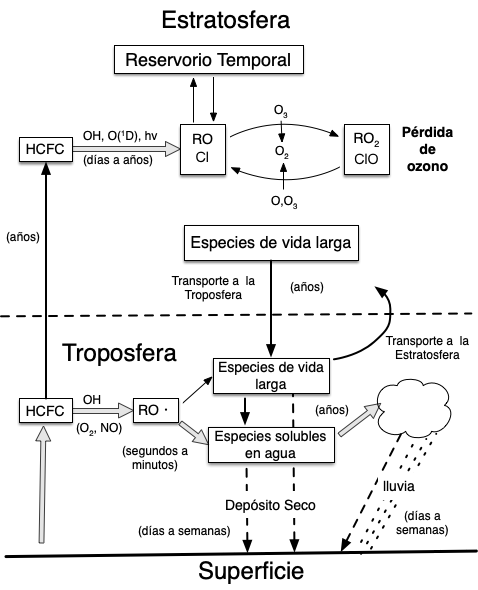
\includegraphics[width=0.95\textwidth]{halogenos_01.png}
\caption{Intercambio de halógenos en la atmósfera.}
\label{halo_01}
\end{center}
\end{figure}

%  
%                 ESTRATOSFERA
%  

\chapter[Quimica de la estatosfera]{Qu\'{\i}mica de la estratosfera}
\index{estratosfera!quimica@química}

El ozono estratosférico (\ce{O3}), descrito previamente en la sección \ref{esozono}, constituye un componente crítico para la biosfera terrestre al absorber el 97-99\% de la radiación ultravioleta (UV-B/C) solar. Su formación y destrucción dinámica, así como su distribución espacial, representan procesos fundamentales para comprender tanto el origen de la vida en el planeta como las amenazas actuales a este escudo protector. Este capítulo aborda los mecanismos químicos que gobiernan su equilibrio natural y las perturbaciones antropogénicas que alteran dicho balance.

En la  Sección~\ref{dvozono}, se analiza la \textbf{distribución vertical y latitudinal del ozono}, caracterizada por:
\begin{itemize}
    \item Máxima concentración entre $20-30 \kilo\metre$\  de altitud (Capa de Ozono)
    \item Variaciones estacionales (agotamiento polar en primavera austral)
    \item Gradientes latitudinales influenciados por la circulación de Brewer-Dobson
\end{itemize}

La Sección~\ref{oestra} explora el \textbf{balance fotoquímico del ozono}, donde se integran las reacciones de Chapman:
\begin{itemize}
    \item Formación: \ce{O2 + h$\nu$ ->[ $\lambda < 242 \nano\metre$] 2O} seguido de \ce{O + O2 ->[M] O3 }
    \item Destrucción natural: \ce{O3 + h$\nu$  ->[$\lambda < 310 \nano\metre$] O2 + O} 
\end{itemize}

La Sección~\ref{cpeoz} detalla los \textbf{ciclos de pérdida catalítica}, mecanismos aceleradores que explican el agotamiento observado desde 1980:
\begin{itemize}
    \item \textbf{Radicales hidroxilo} (\ref{roh}): Ciclo HO$_x$ con reacciones tipo \ce{HO^. + O3 -> HO2^. + O2}
    \item \textbf{Radicales de nitrógeno} (\ref{rno3}): Ciclo NO$_x$ catalizado por \ce{NO^.} de origen natural y antropogénico
    \item \textbf{Radicales de cloro} (\ref{rclo}): Ciclo ClO$_x$ activado por CFCs, con reacciones catalizadas en las superficies de las PSCs (Nubes Estratosféricas Polares)\index{PSC}
\end{itemize}

Finalmente, se discuten las \textbf{unidades Dobson (DU)}, estándar global para cuantificar el ozono total atmosférico, vinculando las mediciones satelitales con los modelos químicos presentados. Estos conceptos, junto con los efectos en salud descritos en \ref{o3_salud}, proveen un marco integral para evaluar políticas de protección de la capa de ozono y mitigación de sustancias agotadoras.

\section{Distribución de ozono}
\label{dvozono}
Los gradientes latitudinales de ozono estratosférico están profundamente influenciados por la \textbf{circulación de Brewer-Dobson},\index{circulacion@circulaci\'on!Brewer-Dobson} un sistema de transporte meridional que domina la dinámica de la estratosfera. Este patrón de circulación, impulsado por ondas planetarias y turbulencia en la tropopausa, transporta masa y especies químicas desde los trópicos hacia los polos en dirección vertical y horizontal. El ozono (\ce{O3}), producido principalmente en la estratosfera tropical por fotólisis de \ce{O2} reacción: \ce{O2 + h$\nu$ -> 2O} ($\lambda < 242\nano\metre$), es arrastrado hacia latitudes medias y polares mediante este mecanismo. Sin embargo, la eficiencia del transporte varía estacionalmente, siendo más intenso durante el invierno y primavera boreales, lo que explica:

\begin{itemize}
    \item Máximas concentraciones de ozono en latitudes altas ($>60^\circ$), excepto en la Antártida durante la primavera austral debido al agujero polar (ver Sección \ref{esozono}).
    \item Un gradiente de concentración decreciente desde los polos hacia el ecuador en capas superiores ($\sim30 \kilo\metre$), invertido en capas bajas ($\sim15 \kilo\metre$) por procesos de destrucción catalítica.
    \item Asimetrías hemisféricas: mayores valores en el hemisferio norte por interacciones con ondas orográficas y mayor actividad de ondas planetarias.
\end{itemize}

La ecuación de continuidad para el ozono estratosférico refleja este balance:
\begin{equation}
\frac{\partial [\ce{O3}]}{\partial t} = P - L - \nabla \cdot (\vec{v}[\ce{O3}])
\end{equation}
donde \( P \) y \( L \) son las tasas de producción y pérdida química, y \( \nabla \cdot (\vec{v}[\ce{O3}]) \) representa el transporte advectivo por la circulación de Brewer-Dobson. Este mecanismo no solo distribuye el ozono, sino que también modula la exposición a UV-B en superficie, con implicaciones climáticas y biológicas globales.

El ozono (\ce{O3}) es una molécula relativamente inestable formada por tres átomos de oxígeno (O) ver \textbf{Figura~\ref{reso3}}. Aunque representa sólo una pequeña fracción de la atmósfera, el ozono es crucial para la vida en la Tierra.
\begin{figure}[htbp]
\begin{center}
\ce{O\bond{=}O\bond{-}O <--> O\bond{-}O\bond{=}O } 
\caption{Molécula de ozono y su resonancia}
\label{reso3}
\end{center}
\end{figure}


Dependiendo de dónde resida el ozono, puede proteger o dañar la vida en la Tierra. La mayor parte del ozono reside en la estratosfera (una capa de la atmósfera entre $10$ y $40\kilo\metre$  por encima de nosotros), donde actúa como un escudo para proteger la superficie de la Tierra de la dañina radiación ultravioleta del Sol. Con un debilitamiento de este escudo, seríamos más susceptibles al cáncer de piel, cataratas y sistemas inmunológicos deteriorados. Más cerca de la Tierra, en la troposfera (la capa atmosférica desde la superficie hasta unos $10\kilo\metre$), el ozono es un contaminante nocivo que daña el tejido pulmonar y las plantas.

\section{Balance de ozono en la estratosfera}\label{oestra}
\index{ozono!estratosfera}

En la estratosfera, el ozono se crea principalmente por la radiación ultravioleta. Cuando los rayos ultravioleta de alta energía inciden en las moléculas de oxígeno ordinarias (\ce{O2}), las dividen en dos átomos de oxígeno únicos, conocidos como oxígeno atómico.
\reaction{ O2 + h$\nu$ -> 2O^. \label{OE1}}
\reaction{ O2 + O^. -> O3  \label{OE2}}
 Luego, un átomo de oxígeno liberado se combina con otra molécula de oxígeno para formar una molécula de ozono. Hay tanto oxígeno en nuestra atmósfera que estos rayos ultravioleta de alta energía son completamente absorbidos en la estratosfera.

El ozono es extremadamente valioso ya que absorbe una variedad de energía ultravioleta. Cuando una molécula de ozono absorbe incluso radiación ultravioleta de baja energía, se divide en una molécula de oxígeno ordinaria y un átomo de oxígeno libre. Por lo general, este átomo de oxígeno libre se vuelve a unir rápidamente con una molécula de oxígeno para formar otra molécula de ozono. Debido a este ´´ciclo ozono-oxígeno'', la  radiación ultravioleta dañina se convierte continuamente en calor.
\reaction{ O3 + h$\nu$ -> O2 +2O^. \label{OE3}}
\reaction*{  O^. + O2 ->  O3  }
Las reacciones naturales distintas del ``ciclo ozono-oxígeno'' descrito anteriormente también afectan la concentración de ozono en la estratosfera. Debido a que el ozono y los átomos de oxígeno libres son muy inestables, reaccionan muy fácilmente con los compuestos de nitrógeno, hidrógeno, cloro y bromo que se encuentran naturalmente en la atmósfera de la Tierra (liberados tanto de fuentes terrestres como oceánicas). Por ejemplo, los átomos individuales de cloro pueden convertir el ozono en moléculas de oxígeno y esta pérdida de ozono equilibra la producción de ozono mediante rayos ultravioleta de alta energía que inciden en las moléculas de oxígeno.
\begin{eqnarray*}
 &\ce{Cl + O3 & -> ClO + O2  \\
 &ClO +  O^.  & -> Cl + O2 }\\ 
  \mathrm{Neto: } &\ce{O3 + O^.  &  -> 2O2}
\end{eqnarray*}
Además del equilibrio natural del ozono, los científicos han descubierto que los niveles de ozono cambian periódicamente como parte de ciclos naturales regulares, como el cambio de estaciones, los vientos y las variaciones solares a largo plazo. Además, las erupciones volcánicas pueden inyectar materiales en la estratosfera que pueden provocar una mayor destrucción del ozono.

A lo largo de la vida de la Tierra, los procesos naturales han regulado el equilibrio del ozono en la estratosfera. Una forma sencilla de comprender el equilibrio del ozono es pensar en un balde que gotea. Siempre que se vierta agua en el balde al mismo ritmo que se escapa, la cantidad o el nivel de agua en el balde seguirá siendo el mismo. Del mismo modo, mientras el ozono se cree al mismo ritmo que se destruye, la cantidad total de ozono seguirá siendo la misma.

Sin embargo, a partir de principios de los años 1970, los científicos encontraron pruebas de que las actividades humanas estaban alterando el equilibrio del ozono. La producción humana de sustancias químicas que contienen cloro, como los clorofluorocarbonos (CFC), ha añadido un factor adicional que destruye el ozono. Los CFC son compuestos formados por cloro, flúor y carbono unidos entre sí. Debido a que son moléculas extremadamente estables, los CFC no reaccionan fácilmente con otras sustancias químicas de la atmósfera inferior. Una de las pocas fuerzas que pueden romper las moléculas de CFC es la radiación ultravioleta. En la atmósfera inferior, los CFC están protegidos de la radiación ultravioleta por la propia capa de ozono. De este modo, las moléculas de CFC pueden migrar intactas a la estratosfera. Aunque las moléculas de CFC son más pesadas que el aire, las corrientes de aire y los procesos de mezcla de la atmósfera las transportan a la estratosfera.

Una vez en la estratosfera, las moléculas de CFC ya no están protegidas de la radiación ultravioleta por la capa de ozono. Bombardeadas por la energía ultravioleta del sol, las moléculas de CFC se descomponen y liberan átomos de cloro. Luego, los átomos de cloro libre reaccionan con las moléculas de ozono, tomando un átomo de oxígeno para formar monóxido de cloro y dejando una molécula de oxígeno ordinaria.

Si cada átomo de cloro liberado por una molécula de CFC destruyera sólo una molécula de ozono, los CFC representarían muy poca amenaza para la capa de ozono. Sin embargo, cuando una molécula de monóxido de cloro encuentra un átomo libre de oxígeno, el átomo de oxígeno rompe el monóxido de cloro, roba el átomo de oxígeno y libera el átomo de cloro nuevamente a la estratosfera para destruir más ozono. Esta reacción ocurre una y otra vez, permitiendo que un solo átomo de cloro actúe como catalizador, destruyendo muchas moléculas de ozono.

Afortunadamente, los átomos de cloro no permanecen en la estratosfera para siempre. Cuando un átomo de cloro libre reacciona con gases como el metano (\ce{CH4}), se une a una molécula de cloruro de hidrógeno (HCl), que puede transportarse hacia abajo desde la estratosfera hasta la troposfera, donde puede ser arrastrado por la lluvia. Por lo tanto, si los humanos dejan de colocar CFC y otras sustancias químicas que destruyen la capa de ozono en la estratosfera, la capa de ozono eventualmente podría repararse a sí misma.

\section[Ciclos de perdida catalitica]{Ciclos de pérdida catalítica}
\label{cpeoz}

\subsection{Radicales hidroxilo}\index{radical!hidroxilo}
\label{roh}

Se encubrió en 1950s que los ciclos iniciados or la oxidación del vapor de agua puede representan un sumidero importante de ozono en la estratosfera. El vapor de agua se suministra a la estratosfera por el transporte y oxidación del metano (\ce{CH4}). El vapor de agua en estratosfera es relativamente uniforme, en el intervalo de $3--5$ ppm. En la estratosfera el vapor de agua se oxida por el \ce{O(^1D)} producido por:
\reaction{H2O + O(^1D)  ->  2OH \label{OHr1}}
Los átomos de alta energía \ce{O(^1D)} son necesario para superar la estabilidad del la molécula de agua.

El radical hidróxido (OH)  producido puede reacciona con el \ce{O3}, produciendo el radial hidroperoxi (\ce{HO2}), el cual reacciona con el \ce{O3}.
\begin{eqnarray*}
& \ce{OH + O3    & -> HO2 + O2 \\
      & HO2 +  O3   &-> OH + 2O2} \\
\mathrm{Neto: } &  \ce{2O3   &  ->  3O2}
\end{eqnarray*}

El conjunto OH y \ce{HO2} se conoce como la familia \ce{HO_$x$}.\index{familia!\ce{HO_$x$}}

Las reacciones anteriores consumen el \ce{O3} conservando el \ce{HO_$x$}. Por lo tanto el \ce{HO_$x$} actúa como catalizador para la pérdida de \ce{O3}. La producción de una molécula de \ce{HO_$x$} puede resultar en la pérdida de un gran minero de moléculas de \ce{O3} por el ciclado del \ce{HO_$x$}. La terminación de este ciclo catalítico requiere de la pérdida del \ce{HO_$x$}, por una reacción como:
\reaction*{OH + HO2 -> H2O + O2}

\subsection{Radicales de nitrógeno}\index{radical!de nitrógeno}\label{rno3}
Un avance en la compresión del  \ce{O3}  estratosférico se obtuvo en los EEUU y otros países involucrados en el lanzamiento de un avión supersónico que volaba en la estratósfera.  Se realizó una evaluación las emisiones de estos aviones en la capa de \ce{O3}.  Un componente importante en la emisión es el óxido nítrico (NO) , formado por al oxidación del \ce{N2} a altas temperatura en el motor del avión. En la estratosfera el NO reacciona rápidamente con el \ce{O3}, para producir  \ce{NO2} , que luego se fotoliza:
\begin{eqnarray*}
 \ce{NO + O3       & -> &NO2 + O2 \\
  NO2 +  h$\nu$  &  -> &NO + O^. \\
   O^. + O2          &  ->[M] & O3}
\end{eqnarray*}


Este ciclo entre el NO y \ce{NO2} tiene lugar en una escala de tiempo de 1 minuto durante el día. No tiene un efecto neto en el \ce{O3} y se denomina como ciclo nulo\index{ozono!ciclo nulo}. Este causa, sin embargo, un intercambio rápido entre el NO y \ce{NO2}. Nos referimos al conjunto de NO y \ce{NO2} como \ce{NO_$x$}.

Investigaciones posteriores de la química del \ce{NO_$x$} en la estratosfera mostraron que una fracción de moléculas de \ce{NO2} reacciona con átomos de oxígeno 

\reaction*{NO2 + O^. -> NO + O2}

La secuencia de reacciones del N representa el ciclo catalítico para la pérdida del ozono \ce{O3} serían:
\begin{eqnarray}
            & \ce{NO + O3     &->   NO2 + O2} \label{R10} \\
            &\ce{NO2 +  O^.   & ->   NO + O2 } \label{R11} \\
  \mathrm{Neto: } &\ce{O3 + O^.  &->  2O2}\nonumber 
\end{eqnarray}

Cada ciclo consume dos moléculas \ce{O_$x$} , que es equivalente a dos moléculas de \ce{O3}. El paso importante es en la velocidad de~\ref{R11}

La terminación del ciclo catalítico involucra la pérdida de los radicales \ce{NO_$x$}. En el día,  \ce{NO_$x$}, se oxida a  \ce{HNO3} por medio de radical OH que es un oxidante fuerte.
\reaction*{NO2 + OH ->[M] HNO3}
Durante la noche el OH esta ausente, debido a que no hay \ce{O(^ID)} para oxidar el \ce{H2O}. La pérdida de  \ce{NO_$x$} durante la noche tiene lugar mediante la oxidación del \ce{NO2} con \ce{O3} y la subsecuente conversión del radical \ce{NO3 } a \ce{N2O5}:
\begin{eqnarray*}
 \ce{NO2 + O3    & ->       & NO3 + O2 \\
       NO3+ NO2  &  ->[M] & N2O5}
\end{eqnarray*}

La formación del \ce{N2O5} sólo tiene lugar durante la noche, debido a que durante el día el \ce{NO3} se fotoliza hacia el \ce{NO2} en una escala de tiempo de unos segundos.

Los productos de oxidación del \ce{NO_$x$}, \ce{HNO3} y \ce{N2O5}, son especies no radicales y tiene un tiempo de vida relativamente largos con respecto a la perdida química (semanas para el \ce{HNO3}, horas a días para el \ce{N2O5}). 
\begin{eqnarray*}
 \ce{HNO3 + h$\nu$   & ->   & NO2 + OH \\
       HNO3 + OH        &  ->  & NO3 + H2O\\
       NO3  + h$\nu$    & ->   & NO2 + O\\
       N2O5 + h$\nu$   & ->   & NO3 + NO2}
\end{eqnarray*}
Estos eventualmente se convierten en óxidos de nitrógeno  \ce{NO_$x$}
y sirven como almacenamiento de \ce{NO_$x$}. Se puede referir al conjunto \ce{NO_$x$} y sus reservas como otras familia química, \ce{NO_$y$}. Finalmente la remoción del \ce{NO_$y$} es por transporte a la troposfera donde el \ce{HNO3} se remueve rápidamente por deposito.\index{familia!\ce{NO_$y$}}

La identificación del mecanismo canalizado por \ce{NO_$x$} para la pérdida de \ce{O3} se volvió una pista crítica para identificar el sumidero faltante del \ce{O3} en el mecanismo de Chapman\index{Chapman@\textbf{Chapman}}.

Trabajos posteriores identificaron que el \ce{N2O}, es un producto de bajo rendimiento de los procesos de nitrificación-desnitrificación, la biosfera es fuente de este compuesto. El \ce{N2O} es una molécula estable que no posee sumideros en la troposfera. Por lo que es transportado a la estratosfera donde se encuentra con las altas concentraciones de \ce{O(^1D)}, permitiendo la oxidación a NO:

\reaction{N2O + O(^1D) -> 2NO}
esta reacción es el 5\% de la pérdida del \ce{N2O}  en la estratosfera; el restante 95\% es convertido a \ce{N2} por la fotólisis y oxidación con  \ce{O(^1D)}  por una via alternativa. Sin embargo, la conversión a \ce{N2} no tiene ningún interés en la química estratosférica.

\subsection{Radicales de cloro}\index{radical!de cloro}\label{rclo}
En 1974, Mario Molina\index{molina@\textbf{Molina, Mario}} y Sherwood Roland\index{sherwood@\textbf{Roland, Sherwood}} indicaron el potencial de la pérdida de \ce{O3} asociada al incremento de las concentraciones atmosféricas de cloroflourocarbonos (CFCs)\index{CFC}\index{cloroflourocarbonos}. Los CFCs no se encuentran en la naturaleza éstos se manufacturan con propósitos industriales en los 1930's  y su uso se incrementó rápidamente en las siguientes décadas. Durante los 1970's y 1980's las concentraciones atmosféricas de los CFCs rozaron 2--4\% al año. Las moléculas de CFC son inertes en la troposfera,  así son transportados a la estratosfera donde se fotolizan y liberan átomos de Cl. Por ejemplo, en el caso de \ce{CF2Cl2} (conocido como CFC-12) \index{CFC-12}
\reaction{CF2Cl2 +  h$\nu$ -> CF2Cl + Cl^.}

Los átomos de Cl  desencadenan el mecanismo de pérdida catalítica para el \ce{O3} involucrando un ciclo entre Cl y ClO (la familia \ce{ClO_$x$})la secuencia es similar a la del mecanismo catalizado con \ce{NO_$x$} (\ref{R11}):
\begin{eqnarray*}
            & \ce{Cl + O3     &->   ClO + O2}  \\
            &\ce{ClO +  O^.   & ->   Cl + O2 }  \\
  \mathrm{Neto: } &\ce{O3 + O^.   &->  2O2} 
\end{eqnarray*}

La terminación de éste ciclo catalítico es mediante la conversión del \ce{ClO_$x$} a un reservorio de cloro no-radical, HCl y \ce{ClNO3}:
\begin{eqnarray*}
 \ce{Cl + CH4   & ->   & HCl + CH3 \\
       ClO + NO2        &  ->[M]  & ClNO3}
\end{eqnarray*}

El tiempo de vida del HCl es típicamente unas pocas semanas y la del \ce{ClNO3} en el orden de un día. Eventualmente estos repertorios se convierten en \ce{ClO_$x$}.
\begin{eqnarray*}
 \ce{HCl + OH   & ->   & Cl + H2O \\
       ClNO3 +   h$\nu$   &  ->  & Cl + NO3}
\end{eqnarray*}
Se define a la familia química \ce{ClO_$y$} como la suma de \ce{ClO_$x$} más sus reservorios.  \index{familia!\ce{ClO_$x$}} 

Molina y Rowland alertaron que la pérdida de \ce{O3}  catalizada con \ce{ClO_$x$}  podría convertirse en una amenaza para la capa de \ce{O3}  en la medida de las concentraciones de CFC se incrementasen. Por sus trabajos relacionados a la pérdida de ozono en la estratosfera y el descubrimiento del hoyo de ozono compartieron el premio Noble de química en 1995 con Paul Crutzen\index{Crutzen@\textbf{Crutzen,Paul}}.

\section{Agotamiento del ozono estratosférico}

El término  ``agotamiento del ozono''\index{ozono!agotamiento} significa más que simplemente la destrucción natural del ozono: significa que la pérdida de ozono excede la creación de ozono (\textbf{Cuadro\,\ref{desozo}}). Piense de nuevo en el ``balde que gotea''. Poner en la atmósfera compuestos adicionales que destruyen el ozono, como los CFC, es como aumentar el tamaño de los agujeros en nuestro ``cubeta'' de ozono. Los agujeros más grandes hacen que el ozono se escape a un ritmo más rápido del que se crea. En consecuencia, disminuye el nivel de ozono que nos protege de la radiación ultravioleta.
\begin{table}[htb]
\caption{Ciclos de destrucción de ozono con halógenos}
\begin{center}
\begin{tabular}{rcl}
\multicolumn{3}{l}{\large\bfseries Ciclo 1 Destrucción de Ozono}\\
\ce{Cl + O3} & \ce{ -> } &\ce{ClO + O2}\\
\ce{ClO + O^. } & \ce{ -> } &\ce{Cl + O2}\\\hline
 Neto: \ce{2O3} & \ce{ -> } & \ce{3O2}\\
\multicolumn{3}{l}{\large\bfseries Ciclo 2}\\
 \ce{ClO + ClO }          & \ce{ -> } &\ce{(ClO)_2}\\
 \ce{(ClO)_2 + h$\nu$ } & \ce{ -> } &\ce{ClOO^. + Cl}\\
 \ce{ClOO^. }                  & \ce{ -> } &\ce{Cl + O2}\\
 \ce{2(Cl + O3 ) }             & \ce{ -> } &\ce{ClO + O2}\\ \hline
 Neto: \ce{2O3} & \ce{ -> } & \ce{3O2}\\
\multicolumn{3}{l}{\large\bfseries Ciclo 3}\\
 \ce{ClO + BrO }          & \ce{ -> } &\ce{Cl + Br + O2}\\
 \ce{BrCl +  h$\nu$ }    & \ce{ -> } &\ce{Cl + Br }\\
 \ce{Cl +  O3 }    & \ce{ -> } &\ce{ClO + O2 }\\
 \ce{Br +  O3 }    & \ce{ -> } &\ce{BrO + O2 }\\\hline
 Neto: \ce{2O3} & \ce{ -> } & \ce{3O2}\\
\end{tabular}
\end{center}
\label{desozo}
\end{table}%
Durante los últimos 15 años se ha descubierto en las zonas de la Antártida y el Ártico un mecanismo adicional que destruye rápidamente el ozono. Sobre los polos de la Tierra durante sus respectivos inviernos, la estratosfera se enfría a temperaturas muy frías y se forman nubes estratosféricas polares (PSC).\index{PSC} En la estratosfera polar, casi todo el cloro se encuentra en forma de gases inactivos o ``de depósito'', como el cloruro de hidrógeno (HCl) y el nitrato de cloro (\ce{ClONO2}), que no reaccionan con el ozono ni entre sí. Sin embargo, las reacciones químicas de estos gases de cloro ``de depósito''  pueden ocurrir en las superficies de las partículas de las nubes estratosféricas polares, convirtiendo los gases de cloro en formas muy reactivas que destruyen rápidamente el ozono. Esta ``química polar'' en las partículas de las nubes estratosféricas ha provocado grandes disminuciones en las concentraciones de ozono sobre la Antártida y el Ártico. De hecho, los niveles de ozono caen tan bajo en primavera sobre la Antártida que los científicos describen esta pérdida como el ``Agujero de Ozono Antártico''.\index{ozono!agujero}

La formación de Nubes estratosféricas se da alrededor de los -72\celsius\, así en el polo sur es más probable que se formen que en el polo norte por las temperaturas que se alcanzan.

Así en las capas donde se tienen nubes estratosféricas polares podemos encontrar que el ozono se ve reducido.

\subsection{Medición de ozono en columna}
La Unidad Dobson\index{unidades!Dobson} (en inglés, DU) es la unidad más común para medir la cantidad presente de ozono en la atmósfera terrestre. Una unidad Dobson es la cantidad de moléculas de ozono que se necesitarían para crear una capa de ozono puro de 0.01 milímetros de espesor a una temperatura de 0 grados Celsius y una presión de 1 atmósfera (la presión del aire en la superficie de la Tierra). Expresado de otra manera, una columna de aire con una concentración de ozono de 1 unidad Dobson contendría aproximadamente $2.69\times10^{16}$ moléculas de ozono en una columna de un centímetro cuadrado de área en la base. Sobre la superficie de la Tierra, el espesor medio de la capa de ozono es de unas 300 unidades Dobson o una capa de 3 milímetros de espesor.

El ozono en la atmósfera no está todo empaquetado en una sola capa a una cierta altitud sobre la superficie de la Tierra; está disperso. Incluso el ozono estratosférico conocido como ``la capa de ozono'' no es una sola capa de ozono puro. Es simplemente una región donde el ozono es más común que en otras altitudes. Los sensores satelitales y otros dispositivos de medición del ozono miden la concentración total de ozono para una columna completa de la atmósfera. La Unidad Dobson es una forma de describir cuánto ozono habría en la columna si estuviera todo comprimido en una sola capa.

La cantidad promedio de ozono en la atmósfera es de aproximadamente 300 unidades Dobson, equivalente a una capa de 3 milímetros de espesor, la altura de 2 centavos apilados. Lo que los científicos llaman el ``agujero'' de ozono antártico es un área donde la concentración de ozono cae a un promedio de aproximadamente 100 unidades Dobson. Cien unidades Dobson de ozono formarían una capa de sólo 1 milímetro de espesor si se comprimieran en una sola capa, aproximadamente de la altura de una moneda de diez centavos.

\textquestiondown Cuánto es esto en comparación con el resto de la atmósfera?  Si todo el aire de una columna vertical que se extiende desde el suelo hasta el espacio fuera recolectado y comprimido a una temperatura de 0 grados Celsius y una presión de 1 atmósfera, esa columna tendría 8 kilómetros de espesor. Al compararse con los 3 milímetros descritos anteriormente y con esto uno se da cuenta de cuán tenue es la capa de ozono de la Tierra.
